\documentclass[10pt,a4paper]{article}
% Preámbulo del informe: paquetes, colores, títulos, código y figuras.

\usepackage[T1]{fontenc}
\usepackage[spanish,es-noquoting,es-tabla]{babel}
\usepackage[a4paper,margin=2.1cm,top=2.3cm,bottom=2.2cm]{geometry}
\usepackage{amsmath,amssymb}
\usepackage{booktabs}
\usepackage{array}
\usepackage{xcolor}
\usepackage{tikz}
\usepackage{float}
\usepackage{listings}
\usepackage{tcolorbox}
\usepackage{enumitem}
\usepackage{fancyhdr}
\usepackage{titlesec}
\usepackage[font=small,labelfont=bf,skip=4pt]{caption}
\usepackage[hidelinks]{hyperref}

\usetikzlibrary{positioning,arrows.meta}
\tcbuselibrary{skins,breakable}

% --- paleta ---------------------------------------------------------------
\definecolor{tinta}{HTML}{1B2733}
\definecolor{acento}{HTML}{1F6FEB}
\definecolor{acentoSuave}{HTML}{DDE9FB}
\definecolor{exito}{HTML}{1A7F37}
\definecolor{exitoSuave}{HTML}{DCF4E3}
\definecolor{gris}{HTML}{6E7781}
\definecolor{grisSuave}{HTML}{F0F2F5}

\color{tinta}

% --- títulos, párrafos y encabezados ---------------------------------------
\titleformat{\section}{\Large\bfseries\color{acento}}{\thesection}{0.7em}{}
\titleformat{\subsection}{\large\bfseries}{\thesubsection}{0.6em}{}
\titlespacing*{\section}{0pt}{14pt}{6pt}
\titlespacing*{\subsection}{0pt}{10pt}{4pt}
\titlespacing*{\paragraph}{0pt}{7pt}{0.8em}
\setlength{\parskip}{4pt}
\setlength{\parindent}{0pt}

\pagestyle{fancy}
\fancyhf{}
\fancyhead[L]{\small\color{gris}Minigestor de base de datos multimodal}
\fancyhead[R]{\small\color{gris}Informe: Partes 1 y 2}
\fancyfoot[C]{\small\color{gris}\thepage}
\renewcommand{\headrulewidth}{0.4pt}

% --- tablas ----------------------------------------------------------------
% Columna de párrafo sin justificar: en celdas estrechas la justificación parte palabras.
\newcolumntype{L}[1]{>{\raggedright\arraybackslash}p{#1}}

% --- código ---------------------------------------------------------------
\lstdefinestyle{consola}{
  basicstyle=\ttfamily\footnotesize,
  keywordstyle=\color{acento}\bfseries,
  commentstyle=\color{gris}\itshape,
  stringstyle=\color{exito},
  numbers=none,
  frame=leftline,
  framesep=8pt,
  rulecolor=\color{acentoSuave},
  framerule=2pt,
  backgroundcolor=\color{grisSuave},
  xleftmargin=10pt,
  breaklines=true,
  showstringspaces=false,
  columns=fullflexible,
  keepspaces=true
}
\lstdefinestyle{sql}{
  style=consola,
  morekeywords={SELECT,FROM,WHERE,CREATE,TABLE,INDEX,USING,ORDER,BY,LIMIT,ON,AND,RTREE}
}
\lstset{style=consola}

% --- cajas y figuras --------------------------------------------------------
\newtcolorbox{resumen}{
  enhanced, colback=exitoSuave, colframe=exito,
  boxrule=0pt, leftrule=3pt, arc=2pt, left=8pt, right=8pt, top=5pt, bottom=5pt}

\tikzset{
  flecha/.style={-{Stealth[length=2mm]}, gris, thick},
}

% Una gráfica de benchmarks/figures con su pie: [ancho]{archivo}{etiqueta}{pie}.
\newcommand{\grafica}[4][\textwidth]{%
  \begin{figure}[!htb]
    \centering
    \includegraphics[width=#1]{../../benchmarks/figures/#2}
    \caption{#4}
    \label{#3}
  \end{figure}}


% --- datos del alumno y del repositorio ---------------------------------------
% Lo único que hay que tocar aquí. Si \codigo queda vacío, su fila no se imprime.
\newcommand{\alumno}{José Huamaní}
\newcommand{\codigo}{}
\newcommand{\carrera}{Ciencias de la Computación, UTEC}
\newcommand{\curso}{Base de Datos 2 (2026-2)}
\newcommand{\entrega}{Entrega parcial, semana 8}
\newcommand{\repositorio}{https://github.com/JoseEd0/project-BD2}

% --- cifras que se sincronizan con el repositorio -------------------------------
% Número de pruebas automáticas y cobertura de líneas y ramas de src/.
\newcommand{\totalpruebas}{1287}
\newcommand{\coberturapruebas}{99}

\begin{document}
\thispagestyle{empty}

{\Huge\bfseries Minigestor de base de datos multimodal\par}
\vspace{2pt}
{\Large Informe incremental: Parte 1 (relacional) y Parte 2 (espacial)\par}
\vspace{8pt}
{\color{acento}\hrule height 1.2pt}
\vspace{8pt}

\begin{tabular}{@{}>{\bfseries\color{gris}}l@{\hspace{1.2em}}l@{}}
Alumno      & \alumno \\
\if\relax\detokenize\expandafter{\codigo}\relax\else
Código      & \codigo \\
\fi
Carrera     & \carrera \\
Curso       & \curso \\
Entrega     & \entrega \\
Repositorio & \href{\repositorio}{\texttt{\repositorio}} \\
\end{tabular}

\vspace{6pt}
\begin{resumen}
Un gestor de base de datos construido desde cero en Python: sin ORM, sin motor externo y
sin librerías que resuelvan las estructuras. Esta entrega cubre la \textbf{Parte~1}
---almacenamiento paginado, índices B+ y hash, algoritmos externos, SQL, transacciones e
interfaz--- y la \textbf{Parte~2}: R-Tree sobre disco, consultas por radio, por cercanía y
por polígono, dos métricas de distancia y panel de mapa. Todo lo que se afirma sobre
rendimiento está \textbf{medido}: tres experimentos reproducibles con un comando, con
resultados crudos y gráficas versionados. El índice espacial se contrastó con PostGIS sobre
100\,000 lugares reales de OpenStreetMap: las 1\,800 consultas devuelven las mismas filas.
\end{resumen}

\section{Diseño arquitectónico}

El sistema es un gestor de base de datos escrito desde cero en Python. \textbf{Ninguna
estructura evaluada se delega en una librería}: las páginas, los árboles, el hash, los
algoritmos externos, el parser y el índice espacial están implementados a mano. Las
dependencias externas se limitan a lo que el enunciado no evalúa: el servidor web
(FastAPI), la interfaz (React, Leaflet), las gráficas y las pruebas.

\begin{center}
\begin{tikzpicture}[
  capa/.style={draw=acento, fill=acentoSuave, rounded corners=2pt, minimum height=6.2mm,
               minimum width=9.6cm, font=\footnotesize},
  base/.style={draw=exito, fill=exitoSuave, rounded corners=2pt, minimum height=6.2mm,
               minimum width=9.6cm, font=\footnotesize},
  nota/.style={font=\scriptsize\itshape, color=gris, anchor=west},
  node distance=1.4mm]
  \node[capa] (ui)  {\texttt{frontend/} \quad React, TypeScript, Leaflet};
  \node[capa, below=of ui]  (api) {\texttt{api/} \quad REST (FastAPI), una sesión por pestaña};
  \node[capa, below=of api] (txn) {\texttt{txn/} \quad sesiones, bloqueos en dos fases, deshacer};
  \node[capa, below=of txn] (qry) {\texttt{sql/} + \texttt{query/} \quad parser, catálogo,
                                   planificador, operadores};
  \node[capa, below=of qry] (idx) {\texttt{index/} \quad B+ agrupado y no agrupado, hash
                                   extendible, R-Tree};
  \node[capa, below=of idx] (ext) {\texttt{external/} \quad ordenamiento, hashing y bucles
                                   anidados externos};
  \node[base, below=of ext] (sto) {\texttt{storage/} \quad registros, páginas, buffer pool,
                                   heap, secuencial};
  \node[base, below=of sto] (spa) {\texttt{spatial/} \quad geometría y métricas (sin
                                   dependencias)};
  \node[nota] at ([xshift=2mm]ui.east)  {HTTP};
  \node[nota] at ([xshift=2mm]txn.east) {aislamiento};
  \node[nota] at ([xshift=2mm]qry.east) {de SQL a filas};
  \node[nota] at ([xshift=2mm]idx.east) {caminos de acceso};
  \node[nota] at ([xshift=2mm]sto.east) {bytes en disco};
\end{tikzpicture}
\end{center}

\textbf{Cada capa solo conoce a la de abajo}: el motor no sabe qué es una transacción ni
que existe un API, y el API no sabe nada de la interfaz. Cuatro decisiones atraviesan todas
las capas:

\begin{itemize}[nosep, leftmargin=*]
  \item \textbf{Todo opera por páginas.} Ninguna estructura abre archivos por su cuenta:
        piden páginas de 4\,096 bytes a un único paginador, con un \emph{buffer pool} LRU
        de 128 páginas. Nada carga un archivo entero en memoria.
  \item \textbf{Registros de tamaño fijo.} La posición de un registro en su página es una
        multiplicación, no una búsqueda; la capacidad de un nodo se \emph{deduce} de dividir
        el tamaño de página entre el de una entrada.
  \item \textbf{Una sola implementación de cada cosa.} La serialización, el manejo de
        páginas y las métricas de distancia viven en un único lugar: una consulta no puede
        dar resultados distintos según el camino que elija el planificador.
  \item \textbf{Nada incrustado.} Tamaño de página, umbrales, abanicos y particiones son
        campos de \texttt{EngineConfig}; rutas y direcciones, variables de entorno; los
        parámetros de los experimentos, argumentos de línea de comandos.
\end{itemize}

\paragraph{El camino de una consulta.} Toda sentencia recorre la misma cadena, y su
resultado lleva, además de las filas, el \textbf{plan de ejecución} con el camino de acceso
elegido y ---con \texttt{EXPLAIN ANALYZE}--- las filas y el tiempo de cada operador.

\begin{center}
\begin{tikzpicture}[
  paso/.style={draw=acento, fill=acentoSuave, rounded corners=2pt, minimum height=7mm,
               font=\scriptsize, align=center, inner sep=3pt},
  node distance=3.5mm]
  \node[paso] (a) {texto\\SQL};
  \node[paso, right=of a] (b) {lexer\\tokens};
  \node[paso, right=of b] (c) {parser\\AST};
  \node[paso, right=of c] (d) {validación\\de tipos};
  \node[paso, right=of d] (e) {planificador\\camino de acceso};
  \node[paso, right=of e] (f) {operadores\\(iteradores)};
  \node[paso, right=of f] (g) {filas\\+ plan};
  \foreach \x/\y in {a/b, b/c, c/d, d/e, e/f, f/g} \draw[flecha] (\x) -- (\y);
\end{tikzpicture}
\end{center}

\paragraph{API e interfaz.} El API expone el motor sin lógica propia: ejecuta guiones SQL,
lista el catálogo, describe la estructura física de una tabla y de sus índices, y crea
tablas a partir de un CSV. Cada pestaña del navegador es una sesión, de modo que dos
pestañas bastan para demostrar bloqueos. La interfaz (figura~\ref{fig:interfaz}) muestra a
la vez los cuatro paneles del enunciado ---archivos, consultas, resultados y plan--- y,
para la Parte~2, un mapa con el resultado, la figura de la consulta y los MBR del R-Tree.

\begin{figure}[!htb]
  \centering
  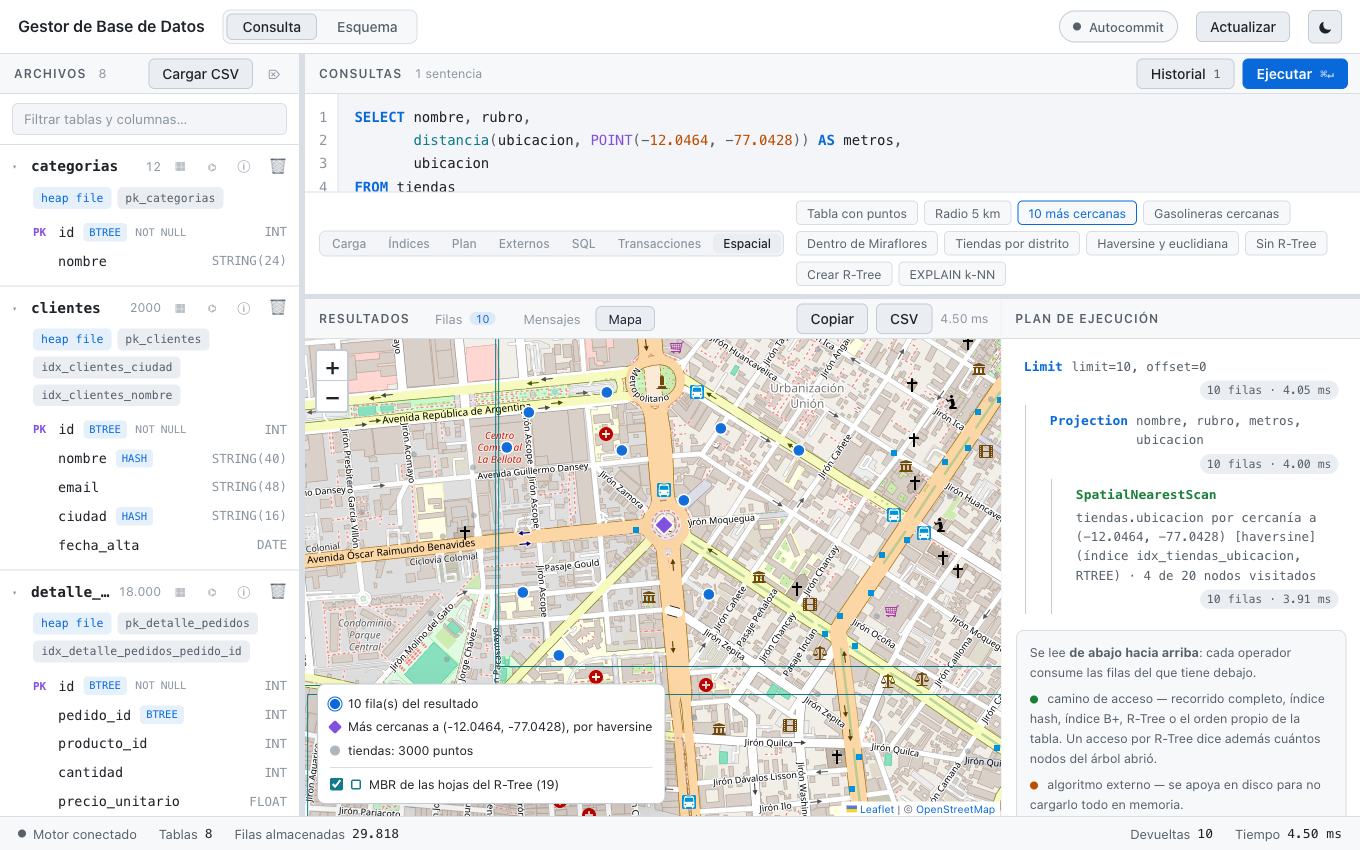
\includegraphics[width=0.94\textwidth]{figuras/interfaz.png}
  \caption{La interfaz tras pedir las 10 tiendas más cercanas a un punto. A la izquierda, los
           archivos con su organización y sus índices; arriba, el editor SQL con los atajos de
           ejemplo; en el centro, el resultado sobre el mapa, con los rectángulos (MBR) de las
           hojas del R-Tree; a la derecha, el plan de ejecución, que usó el índice y abrió 4
           de sus 20 nodos.}
  \label{fig:interfaz}
\end{figure}

\section{Dominio de datos}

Se trabaja con dos conjuntos de datos, uno por cada necesidad.

\paragraph{Un comercio electrónico, generado.} El dataset de demostración modela clientes
que hacen pedidos de productos organizados en categorías, más una red de tiendas con
ubicación en Lima: seis tablas y unas 30\,000 filas. \textbf{Cada tabla usa una organización
física distinta}, para que las diferencias se vean funcionando sobre los mismos datos.

\begin{center}
\small
\begin{tabular}{@{}lrL{5.0cm}ll@{}}
\toprule
\textbf{Tabla} & \textbf{Filas} & \textbf{Columnas} & \textbf{Organización} & \textbf{Índice secundario} \\
\midrule
\texttt{categorias}       & 12      & id, nombre & heap file & --- \\
\texttt{clientes}         & 2\,000  & id, nombre, email, ciudad, fecha\_alta & heap file & hash en \texttt{ciudad} \\
\texttt{productos}        & 800     & id, nombre, categoria\_id, precio, stock & B+ agrupado & --- \\
\texttt{pedidos}          & 6\,000  & id, cliente\_id, fecha, estado, total & archivo secuencial & --- \\
\texttt{detalle\_pedidos} & 18\,000 & id, pedido\_id, producto\_id, cantidad, precio\_unitario & heap file & B+ en \texttt{pedido\_id} \\
\texttt{tiendas}          & 3\,000  & id, nombre, rubro, distrito, ubicacion & heap file & R-Tree en \texttt{ubicacion} \\
\bottomrule
\end{tabular}
\end{center}

Sale de un generador determinista (\texttt{demos/poblar\_ecommerce.py}): la misma semilla
produce los mismos datos byte a byte, su tamaño se ajusta con \texttt{-{}-escala} y los
seis CSV están versionados para cargarlos desde la interfaz. Las tiendas se generan dentro
del contorno de doce distritos, de modo que \guillemotleft{}tiendas dentro de
Miraflores\guillemotright{} tiene una respuesta comprobable.

\paragraph{Lugares reales de OpenStreetMap.} Para la parte espacial importa que los puntos
estén repartidos como en el mundo y no como los reparte un generador. El guion
\texttt{demos/descargar\_lugares.py} descarga los puntos de interés del Perú ---colegios,
restaurantes, farmacias, bancos, gasolineras--- y los deja en un CSV que el gestor carga
tal cual: \texttt{id, nombre, rubro, ubicacion}, con la ubicación como
\texttt{POINT(latitud, longitud)}. Son \textbf{128\,011 lugares} con nombre en todo el país
(26\,606 en Lima y Callao), en 128 rubros. Lee el extracto de Geofabrik pidiendo por HTTP
solo los bytes de las capas que necesita y decodifica el shapefile con un lector propio.
Es el dataset del experimento espacial y el que se usa en la demostración del mapa.

\paragraph{Tipos.} El motor almacena enteros, reales, booleanos, fechas, texto de longitud
fija, bytes y puntos. Al cargar un CSV, el tipo de cada columna se deduce de todos sus
valores. Solo se comparan valores de la misma familia: \texttt{WHERE id = 'abc'} no
devuelve cero filas en silencio, se rechaza nombrando la columna, y antes de leer ninguna
fila.

\section{Explicación de los algoritmos}

\subsection{Almacenamiento: páginas, heap file y archivo secuencial}

Un registro es un mapa de nulos seguido de sus campos, todos de tamaño fijo. Una página de
4\,096 bytes tiene una cabecera de 8 y ranuras de un byte de estado (\emph{libre},
\emph{ocupada} o \emph{lápida}) más el registro: caben
$\lfloor (4096 - 8)/(1 + \text{registro}) \rfloor$.

\paragraph{Heap file.} Los registros se guardan donde haya sitio. La única estructura
auxiliar es una \textbf{lista enlazada de páginas con ranuras libres}: insertar va a la
cabeza de la lista ($O(1)$) y borrar devuelve la página a la lista, que es la reutilización
de espacio que pide el enunciado. No sabe buscar por valor (recorrido completo); para eso
están los índices, cuyas hojas guardan la dirección \texttt{(página, ranura)} de cada fila.

\paragraph{Archivo secuencial.} Los registros se mantienen ordenados por clave en un
\textbf{espacio principal}, con un \textbf{espacio auxiliar} de desbordamiento.
\begin{itemize}[nosep, leftmargin=*]
  \item \emph{Buscar}: búsqueda binaria sobre las páginas ($O(\log P)$), otra dentro de la
        página y, si hace falta, su cadena de desbordamiento.
  \item \emph{Insertar}: si la página tiene sitio, se desplazan sus ranuras; si está llena
        y la clave es la mayor, se añade una página; si va en medio, a la cadena de
        desbordamiento de esa página.
  \item \emph{Borrar}: eliminación \emph{lazy}; se marca una lápida, que conserva la
        posición de la clave.
  \item \emph{Reorganizar}: cuando
        $(\text{lápidas} + \text{desbordamiento}) / \text{registros}$ supera el
        \textbf{30\,\%}, se reescribe el espacio principal en orden, sin lápidas, llenando
        cada página al \textbf{80\,\%}; ese hueco hace que las inserciones siguientes
        quepan en su sitio.
\end{itemize}

\subsection{Índices: B+ y hash extendible}

\paragraph{Árbol B+.} Cada nodo ocupa una página; los datos están solo en las hojas, que
van encadenadas. Si una hoja se desborda se parte por la mitad y la primera clave de la
mitad derecha \emph{se copia} al padre; si un nodo interno se desborda, su clave central
\emph{sube}. Al borrar, un nodo que baja de la mitad pide una entrada a un hermano
(\emph{redistribución}) o se une con él (\emph{fusión}). El árbol solo crece o mengua por
la raíz, así que todas las hojas quedan siempre a la misma profundidad.

\begin{center}
\small
\begin{tabular}{@{}L{3.0cm}L{6.6cm}rr@{}}
\toprule
\textbf{Variante} & \textbf{Qué guardan las hojas} & \textbf{Hoja} & \textbf{Interno} \\
\midrule
Agrupado      & la fila completa: el árbol \emph{es} la tabla, uno por tabla & 50 & 340 \\
No agrupado   & la dirección de la fila en el heap; varios por tabla; la clave es el par
                \texttt{(valor, dirección)}, que admite valores repetidos & 292 & 226 \\
\bottomrule
\end{tabular}

{\footnotesize\color{gris} Entradas por nodo con páginas de 4 KB y una clave entera
(tabla \texttt{productos}, fila de 73 bytes).}
\end{center}

\paragraph{Hash extendible.} Un directorio de $2^{gd}$ punteros (profundidad global $gd$)
apunta a cubetas, cada una con su profundidad local $ld$; una cubeta de profundidad $ld$
recibe exactamente $2^{gd-ld}$ punteros. Buscar son dos accesos, sea cual sea el tamaño.
Cuando una cubeta se llena, si $ld = gd$ se \textbf{duplica el directorio} (se copian
punteros, no se mueve ningún registro) y se parte \textbf{solo esa cubeta} según el bit
$ld$ del hash. Borrar deshace el camino: una cubeta holgada se \textbf{funde con su
gemela} y, si las dos mitades del directorio quedan iguales, este se reduce a la mitad. Si
muchas filas comparten clave, partir no reparte nada: se detecta antes de duplicar y se
encadena una página de desbordamiento. El hash es Blake2b sobre los bytes de la clave,
porque el de Python cambia en cada proceso.

\subsection{Algoritmos externos}

Trabajan con más datos de los que caben en memoria: el presupuesto es un buffer de 16
páginas, y todo lo demás vive en archivos temporales leídos página a página.

\begin{description}[leftmargin=*, nosep]
  \item[\texttt{ORDER BY}: ordenamiento externo.] Se generan \emph{runs} ordenados del
        tamaño del buffer ($\lceil N/B \rceil$) y se mezclan de 8 en 8 con un montículo,
        con una página por run en memoria: $\lceil \log_8 (N/B) \rceil$ pasadas.
  \item[\texttt{GROUP BY} y \texttt{DISTINCT}: hashing externo.] Las filas se reparten en
        16 particiones por el hash de la clave; filas iguales caen en la misma. De cada
        grupo se guarda un \textbf{acumulador} (un contador, una suma compensada, un
        mínimo), no sus filas: la memoria depende del número de grupos, no del de filas.
        Si los grupos de una partición no caben, se vuelve a repartir con otra función de
        hash.
  \item[\texttt{JOIN} con igualdad: \emph{grace hash join}.] Se particionan las dos tablas
        con el mismo hash; para cada par de particiones, una se carga en un diccionario y
        la otra la recorre: $O(N + M)$ en lugar de $O(N \cdot M)$. Admite claves
        compuestas, una condición residual y las cuatro reuniones
        (\texttt{INNER}, \texttt{LEFT}, \texttt{RIGHT}, \texttt{FULL}).
  \item[\texttt{JOIN} sin igualdad: bucles anidados en bloques.] Sin una clave por la que
        repartir, se compara todo con todo, pero la tabla interior se relee una vez por
        \emph{bloque} de la exterior y no una vez por fila. Es también la salida del hash
        join para una clave tan repetida que ningún hash la separa.
\end{description}

\subsection{Procesamiento de consultas y transacciones}

El parser es recursivo descendente, con las precedencias completas de expresiones, y
señala cada error con línea, columna y un cursor. El planificador elige por reglas el
\textbf{camino de acceso} mirando las condiciones del \texttt{WHERE}, y el ejecutor sigue
el modelo de iteradores (\emph{Volcano}): cada operador pide filas a su hijo.

\begin{center}
\small
\begin{tabular}{@{}L{5.4cm}L{5.6cm}L{4.0cm}@{}}
\toprule
\textbf{En la consulta} & \textbf{Con una estructura que lo resuelva} & \textbf{Sin ella} \\
\midrule
\texttt{col = valor}                 & \texttt{IndexLookup} (hash, B+, R-Tree)      & \texttt{SequentialScan} \\
\texttt{col BETWEEN a AND b}         & \texttt{IndexRange}, \texttt{PrimaryKeyRange} & \texttt{SequentialScan} \\
\texttt{ORDER BY clave}              & \texttt{OrderedScan}: la tabla ya está en orden & \texttt{ExternalSort} \\
\texttt{distancia(col, p) < r}       & \texttt{SpatialRangeScan}                     & recorrido + filtro \\
\texttt{intersecta(col, polígono)}   & \texttt{SpatialPolygonScan}                   & recorrido + filtro \\
\texttt{ORDER BY distancia(col, p)}  & \texttt{SpatialNearestScan}, sin ordenar      & recorrido + \texttt{ExternalSort} \\
\bottomrule
\end{tabular}
\end{center}

Una consulta mal escrita se rechaza \textbf{antes de leer ninguna fila}, también sobre una
tabla vacía: columnas inexistentes, una constante de otro tipo que su columna, una función
mal llamada o un \texttt{SUM} sobre texto. Y una sentencia que falla a mitad no deja nada
escrito: \texttt{INSERT} y \texttt{UPDATE} validan todas las filas antes de escribir la
primera.

\paragraph{Transacciones.} \texttt{BEGIN TRANSACTION} \dots{} \texttt{END TRANSACTION}
agrupa sentencias. Los bloqueos son por tabla, compartidos para leer y exclusivos para
escribir, y se sueltan todos al confirmar o abortar: \textbf{bloqueo en dos fases}. Antes
de esperar un bloqueo se recorre el \textbf{grafo de espera}; si esperar cerraría un ciclo,
esa transacción aborta y la otra continúa. Abortar recorre el registro de cambios
\emph{al revés} aplicando el inverso de cada uno. El guion \texttt{demos/concurrencia.py}
lo demuestra con hilos: cuatro hilos restan 25 veces de un saldo de 1\,000 y sin control
queda en 975 en lugar de 900 (una \emph{race condition} real); con transacciones, siempre
900; y dos transacciones que piden dos tablas en orden opuesto terminan en un interbloqueo
que el gestor detecta, abortando exactamente una.

\subsection{Base de datos espacial: R-Tree}

\paragraph{Métricas.} Un punto es \texttt{POINT(latitud, longitud)}. La distancia
\textbf{euclidiana} es la recta sobre el plano de coordenadas, en grados; la de
\textbf{Haversine}, el arco sobre la esfera, en metros:
\[
d = 2R \arcsin\sqrt{\sin^2\!\tfrac{\Delta\varphi}{2} + \cos\varphi_1 \cos\varphi_2
    \sin^2\!\tfrac{\Delta\lambda}{2}}, \qquad R = 6\,371\,008.8 \text{ m}
\]
Cada métrica ofrece además la \textbf{distancia mínima de un punto a un rectángulo}, que es
lo que el índice necesita para descartar ramas enteras sin leerlas.

\paragraph{Estructura.} Es el R-Tree de Guttman (1984) sobre disco. Una hoja guarda hasta
185 puntos con la dirección de su fila; un nodo interno, hasta 113 hijos, cada uno con su
\textbf{MBR}: el menor rectángulo que encierra todo lo que cuelga de él. A diferencia del
B+, los MBR de dos hermanos pueden solaparse, así que la calidad del árbol depende de que
queden pequeños.
\begin{itemize}[nosep, leftmargin=*]
  \item \emph{Insertar}: se baja por el hijo cuyo MBR \emph{menos crece}; si la hoja se
        desborda, se divide y los MBR del camino se ajustan.
  \item \emph{Dividir (cuadrática)}: las dos entradas que más área desperdiciarían juntas
        son las semillas; el resto se asigna de una en una, empezando por la de
        preferencia más marcada. Los empates de área ---puntos alineados--- se resuelven
        por semiperímetro.
  \item \emph{Borrar}: un nodo que baja del 40\,\% se disuelve y sus entradas se
        reinsertan, porque los hermanos de un R-Tree no tienen un orden que permita
        fusionarlos.
  \item \emph{Carga masiva (STR)}: \texttt{CREATE INDEX} sobre una tabla con datos ordena
        los puntos por latitud, los corta en franjas, ordena cada franja por longitud y la
        corta en hojas que no se solapan. Reutiliza el ordenamiento externo de la Parte~1.
\end{itemize}

\paragraph{Las tres búsquedas.}
\begin{description}[leftmargin=*, nosep]
  \item[Por radio.] Solo se abren los hijos cuya distancia mínima al centro no supera el
        radio; en las hojas se mide la distancia exacta.
  \item[$k$ vecinos más cercanos.] Búsqueda \emph{primero-el-mejor} (Hjaltason y Samet,
        1999): una cola de prioridad mezcla nodos, con la distancia mínima a su MBR, y
        puntos, con su distancia real. Se saca siempre lo más cercano; si es un punto,
        \textbf{es el siguiente vecino}, porque nada de lo que queda puede estar más cerca.
        Es incremental: el \texttt{LIMIT} deja de pedir tras el $k$-ésimo y no se ordena
        nada.
  \item[Por polígono.] \emph{Filtrar y refinar}: el árbol busca por el rectángulo que
        encierra al polígono y cada candidato pasa la prueba exacta de punto en polígono
        (regla par-impar). Admite polígonos cóncavos.
\end{description}

\begin{lstlisting}[style=sql]
CREATE INDEX idx_lugares ON lugares USING RTREE (ubicacion);
SELECT * FROM lugares WHERE distancia(ubicacion, POINT(-12.0464, -77.0428)) < 5000;
SELECT * FROM lugares ORDER BY distancia(ubicacion, POINT(-12.0464, -77.0428)) LIMIT 10;
SELECT * FROM lugares WHERE intersecta(ubicacion,
                            POLYGON((-12.11, -77.05), (-12.11, -77.01), (-12.14, -77.01)));
\end{lstlisting}

Las funciones espaciales se evalúan como cualquier expresión, de modo que las tres
consultas dan \textbf{lo mismo con índice que sin él}; con el R-Tree, el plan dice además
cuántos nodos del árbol abrió.

\section{Parte experimental}

\subsection{Metodología}

\textbf{Todo se mide; nada se estima.} Cada experimento es un guion que se ejecuta con un
comando, recibe sus parámetros por línea de comandos ---tamaños, número de consultas,
semilla--- y guarda sus resultados crudos en \texttt{benchmarks/results/}; de esos archivos
salen las gráficas y \emph{todas las cifras de esta sección}. Los tamaños son los del
enunciado: tablas de 1\,000, 10\,000 y 100\,000 registros. Las técnicas comparadas reciben
los mismos datos y las mismas consultas. Entorno: macOS, Python~3.12, páginas de 4~KB; para
el experimento espacial, PostgreSQL~17 con PostGIS~3.6.

\begin{lstlisting}
python -m benchmarks.storage_benchmark --sizes 1000 10000 100000 --queries 100
python -m benchmarks.index_benchmark   --sizes 1000 10000 100000 --queries 100
python -m benchmarks.spatial_benchmark --sizes 1000 10000 100000 --queries 100 \
       --points-file data/datasets/lugares_peru.csv
\end{lstlisting}

\begin{resumen}
\textbf{Cómo leer las gráficas y las tablas.}
\begin{itemize}[nosep, leftmargin=*]
  \item Cada gráfica tiene un panel por operación. El eje horizontal es el \textbf{tamaño de
        la tabla} (1\,000, 10\,000 y 100\,000 filas); el vertical, lo que se mide, con su
        unidad: \textbf{ms} son milisegundos y \textbf{KiB}, kibibytes (1\,024 bytes). Hay una
        línea por técnica, y \textbf{cuanto más abajo, mejor}.
  \item Los dos ejes son \textbf{logarítmicos}: cada marca vale diez veces la anterior. Una
        línea plana significa que el coste no depende del tamaño; una que sube en diagonal,
        que crece en proporción a él.
  \item El número escrito al final de cada línea es su valor con la tabla de 100\,000 filas.
        Las tablas traen los tres tamaños; en negrita va el mejor valor de cada columna.
\end{itemize}
\end{resumen}

\subsection{Experimento 1: heap file frente a archivo secuencial}

Sobre la misma tabla se mide cuánto tarda insertar todas las filas, cuánto tardan 100
búsquedas por clave primaria, cuánto ocupa el archivo y cuánto tarda reorganizarlo
(figura~\ref{fig:almacenamiento} y tabla~\ref{tab:almacenamiento}).

\grafica[0.78\textwidth]{almacenamiento.png}{fig:almacenamiento}{Heap file frente a archivo
secuencial. En la búsqueda se ve el cruce: el heap sube en diagonal y el secuencial es casi
plano.}

\begin{table}[H]
\centering
\caption{Heap file frente a archivo secuencial. Tiempos en milisegundos (ms) y espacio en KiB: \textbf{menos es mejor}, y en negrita va el mejor valor de cada tamaño.}\label{tab:almacenamiento}
\small
\begin{tabular}{@{}llrrr@{}}
\toprule
 & & \multicolumn{3}{c}{\textbf{Número de filas de la tabla}} \\
\cmidrule(lr){3-5}
\textbf{Operación} & \textbf{Técnica} & \textbf{1\,000} & \textbf{10\,000} & \textbf{100\,000} \\
\midrule
Insertar todas las filas & heap file & \textbf{7.66} & \textbf{71.8} & \textbf{744} \\
{\footnotesize\color{gris}tiempo total, en ms} & archivo secuencial & 25.3 & 265 & 3\,838 \\
\addlinespace[3pt]
100 búsquedas por clave & heap file & \textbf{1.08} & 10.6 & 97.2 \\
{\footnotesize\color{gris}tiempo total, en ms} & archivo secuencial & 4.62 & \textbf{4.54} & \textbf{5.74} \\
\addlinespace[3pt]
Espacio que ocupa el archivo & heap file & \textbf{64.0} & \textbf{576} & \textbf{5\,720} \\
{\footnotesize\color{gris}en KiB} & archivo secuencial & 100 & 964 & 9\,608 \\
\addlinespace[3pt]
Reorganizar el archivo {\footnotesize\color{gris}(ms)} & archivo secuencial & 2.63 & 19.3 & 194 \\
\bottomrule
\end{tabular}
\end{table}

\begin{itemize}[nosep, leftmargin=*]
  \item \textbf{El cruce está entre 1\,000 y 10\,000 filas.} Con 1\,000 registros, recorrer el
        heap entero (1.08 ms las 100 búsquedas) gana a la búsqueda binaria del secuencial
        (4.62 ms). A partir de ahí el heap crece de forma lineal y el secuencial casi no se
        mueve: con 100\,000 filas \textbf{el secuencial busca 17 veces más rápido}.
  \item \textbf{El orden se paga al escribir.} Insertar cuesta 5.2 veces más en el secuencial:
        cada inserción localiza su página y desplaza bytes, y cada tanto se dispara una
        reorganización.
  \item \textbf{El secuencial ocupa 1.7 veces más}, y es deliberado: el factor de llenado del
        80\,\% deja hueco para las inserciones futuras.
  \item \textbf{Cuándo usar cada uno:} heap si se escribe mucho y se consulta por índice;
        secuencial si se consulta por clave o por rango y las escrituras son la minoría.
\end{itemize}

\subsection{Experimento 2: B+ agrupado, B+ no agrupado y hash extendible}

Se mide cuánto tarda construir el índice, 100 búsquedas por igualdad, 100 consultas por
rango, recorrer la tabla entera en orden, y borrar y reinsertar el 10\,\% de las filas; y
cuánto ocupa (figura~\ref{fig:indices} y tabla~\ref{tab:indices}). Las búsquedas de los
índices no agrupados \textbf{incluyen el salto al heap}, que es el coste real de usarlos.

\grafica{indices.png}{fig:indices}{B+ agrupado, B+ no agrupado y hash extendible. En el
rango y en el recorrido ordenado falta la línea del hash: no puede hacer ninguna de las dos
cosas.}

\begin{table}[H]
\centering
\caption{Los tres índices. Tiempos en milisegundos (ms) y espacio en KiB: \textbf{menos es mejor}, y en negrita va el mejor valor de cada tamaño. \emph{No soportado}: la técnica no puede resolver esa operación.}\label{tab:indices}
\small
\begin{tabular}{@{}llrrr@{}}
\toprule
 & & \multicolumn{3}{c}{\textbf{Número de filas de la tabla}} \\
\cmidrule(lr){3-5}
\textbf{Operación} & \textbf{Técnica} & \textbf{1\,000} & \textbf{10\,000} & \textbf{100\,000} \\
\midrule
Construir el índice & B+ agrupado & 32.6 & 584 & 9\,259 \\
{\footnotesize\color{gris}tiempo total, en ms} & B+ no agrupado & 319 & 3\,790 & 49\,742 \\
 & hash extendible & \textbf{27.1} & \textbf{339} & \textbf{3\,464} \\
\addlinespace[3pt]
100 búsquedas por igualdad & B+ agrupado & \textbf{1.72} & \textbf{6.23} & \textbf{7.98} \\
{\footnotesize\color{gris}tiempo total, en ms} & B+ no agrupado & 23.9 & 24.2 & 33.6 \\
 & hash extendible & 12.5 & 9.59 & 11.1 \\
\addlinespace[3pt]
100 consultas por rango & B+ agrupado & \textbf{3.41} & \textbf{8.66} & \textbf{11.0} \\
{\footnotesize\color{gris}tiempo total, en ms} & B+ no agrupado & 34.3 & 36.3 & 53.5 \\
 & hash extendible & \multicolumn{3}{c}{\emph{no soportado}} \\
\addlinespace[3pt]
Recorrer toda la tabla en orden & B+ agrupado & \textbf{0.31} & \textbf{3.50} & \textbf{36.9} \\
{\footnotesize\color{gris}tiempo total, en ms} & B+ no agrupado & 2.13 & 22.8 & 390 \\
 & hash extendible & \multicolumn{3}{c}{\emph{no soportado}} \\
\addlinespace[3pt]
Borrar y reinsertar el 10\,\% & B+ agrupado & \textbf{7.61} & 174 & 2\,295 \\
{\footnotesize\color{gris}tiempo total, en ms} & B+ no agrupado & 79.5 & 911 & 9\,622 \\
 & hash extendible & 15.0 & \textbf{111} & \textbf{1\,464} \\
\addlinespace[3pt]
Espacio que ocupa el índice & B+ agrupado & 100 & 924 & 9\,312 \\
{\footnotesize\color{gris}en KiB} & B+ no agrupado & \textbf{24.0} & \textbf{220} & 2\,060 \\
 & hash extendible & 28.0 & 264 & \textbf{2\,056} \\
\bottomrule
\end{tabular}
\end{table}

\begin{itemize}[nosep, leftmargin=*]
  \item \textbf{El B+ agrupado gana en consultas.} Responde 100 igualdades en
        7.98 ms con 100\,000 filas porque la fila ya está en la hoja. El hash tarda
        11.1 ms pese a ser $O(1)$: toda la diferencia es el salto al heap. El B+ no agrupado
        (33.6 ms) suma $O(\log N)$ \emph{más} el salto.
  \item \textbf{El salto al heap domina cuando hay muchos resultados.} Recorrer en orden
        100\,000 filas tarda 36.9 ms en el agrupado y 390 ms en el no agrupado:
        11 veces más con la misma estructura. La diferencia son 100\,000 accesos sueltos.
  \item \textbf{El hash gana al escribir} ---construye 14 veces más rápido que el B+ no
        agrupado y es el más rápido borrando y reinsertando--- \textbf{pero no admite rangos ni
        orden}: no es un cero de rendimiento, es una limitación de la técnica.
  \item \textbf{El espacio va al revés.} El agrupado ocupa 4.5 veces más que los otros dos
        porque guarda las filas; por eso solo puede haber uno por tabla y tantos secundarios
        como haga falta.
  \item \textbf{Cuándo usar cada uno:} agrupado para la clave primaria; hash para columnas que
        solo se consultan por igualdad; B+ no agrupado cuando además hacen falta rangos.
\end{itemize}

\subsection{Experimento 3: búsqueda secuencial, R-Tree y GiST de PostgreSQL}

Las tres técnicas responden las mismas consultas sobre los mismos puntos: \textbf{lugares
reales de OpenStreetMap} del Perú, de los que se toman muestras de 1\,000, 10\,000 y
100\,000. Las consultas son las del enunciado: los lugares a menos de 1, 5 y 10~km de un
punto, y los 10, 50 y 100 más cercanos a él; cien de cada una, centradas junto a puntos de
la muestra. Las dos técnicas del motor se miden con el mismo SQL de punta a punta; GiST, con
PostGIS sobre una columna \texttt{geography}, \texttt{ST\_DWithin} y el operador
\texttt{<->}.

\paragraph{Antes de medir: \textquestiondown{}responden lo mismo?} Un índice que acelera cambiando la
respuesta no es una comparación. El experimento aborta si el R-Tree devuelve filas distintas
de las del recorrido, y anota cuántas consultas de PostGIS coinciden con el motor:
\textbf{las 1\,800 consultas coinciden, fila por fila}, y PostgreSQL confirma con
\texttt{EXPLAIN} que usa el índice en todas.

\grafica{espacial-radio.png}{fig:radio}{Consultas por radio. La línea del recorrido
secuencial es la misma en los tres paneles: no depende del radio.}

\begin{table}[H]
\centering
\caption{Consultas por radio: tiempo medio de \emph{una} consulta, en milisegundos (promedio de 100). Menos es mejor; en negrita, el mejor valor de cada tamaño. La última columna es cuántos lugares devuelve de media cada consulta sobre la tabla de 100\,000.}\label{tab:radio}
\small
\begin{tabular}{@{}llrrrr@{}}
\toprule
 & & \multicolumn{3}{c}{\textbf{Número de puntos de la tabla}} & \\
\cmidrule(lr){3-5}
\textbf{Consulta} & \textbf{Técnica} & \textbf{1\,000} & \textbf{10\,000} & \textbf{100\,000} & \textbf{Lugares devueltos} \\
\midrule
A menos de 1 km & búsqueda secuencial & 3.67 & 34.5 & 353 & 64.1 \\
{\footnotesize\color{gris}tiempo por consulta, en ms} & R-Tree & 0.25 & 0.40 & 1.07 & \\
 & GiST (PostgreSQL) & \textbf{0.051} & \textbf{0.045} & \textbf{0.25} & \\
\addlinespace[3pt]
A menos de 5 km & búsqueda secuencial & 3.60 & 34.4 & 357 & 544 \\
{\footnotesize\color{gris}tiempo por consulta, en ms} & R-Tree & 0.29 & 0.75 & 5.49 & \\
 & GiST (PostgreSQL) & \textbf{0.045} & \textbf{0.061} & \textbf{0.50} & \\
\addlinespace[3pt]
A menos de 10 km & búsqueda secuencial & 3.63 & 34.9 & 353 & 1\,577 \\
{\footnotesize\color{gris}tiempo por consulta, en ms} & R-Tree & 0.38 & 1.30 & 11.5 & \\
 & GiST (PostgreSQL) & \textbf{0.051} & \textbf{0.10} & \textbf{1.00} & \\
\bottomrule
\end{tabular}
\end{table}

\grafica{espacial-knn.png}{fig:knn}{Vecinos más cercanos. El R-Tree y GiST son casi planos:
su coste apenas depende del tamaño de la tabla.}

\begin{table}[H]
\centering
\caption{Vecinos más cercanos: tiempo medio de \emph{una} consulta, en milisegundos (promedio de 100). Menos es mejor; en negrita, el mejor valor de cada tamaño.}\label{tab:knn}
\small
\begin{tabular}{@{}llrrr@{}}
\toprule
 & & \multicolumn{3}{c}{\textbf{Número de puntos de la tabla}} \\
\cmidrule(lr){3-5}
\textbf{Consulta} & \textbf{Técnica} & \textbf{1\,000} & \textbf{10\,000} & \textbf{100\,000} \\
\midrule
Los 10 más cercanos & búsqueda secuencial & 7.75 & 75.6 & 1\,302 \\
{\footnotesize\color{gris}tiempo por consulta, en ms} & R-Tree & 0.31 & 0.42 & 0.64 \\
 & GiST (PostgreSQL) & \textbf{0.058} & \textbf{0.056} & \textbf{0.13} \\
\addlinespace[3pt]
Los 50 más cercanos & búsqueda secuencial & 8.02 & 76.2 & 1\,304 \\
{\footnotesize\color{gris}tiempo por consulta, en ms} & R-Tree & 0.49 & 0.65 & 1.02 \\
 & GiST (PostgreSQL) & \textbf{0.10} & \textbf{0.096} & \textbf{0.21} \\
\addlinespace[3pt]
Los 100 más cercanos & búsqueda secuencial & 8.14 & 76.1 & 1\,308 \\
{\footnotesize\color{gris}tiempo por consulta, en ms} & R-Tree & 0.73 & 0.97 & 1.37 \\
 & GiST (PostgreSQL) & \textbf{0.12} & \textbf{0.13} & \textbf{0.28} \\
\bottomrule
\end{tabular}
\end{table}

\paragraph{Por qué: los nodos que abre cada consulta.} El plan de ejecución dice cuántos
nodos del R-Tree visitó cada búsqueda (figura~\ref{fig:nodos} y tabla~\ref{tab:nodos}). El árbol pasa de 8 a
610 nodos, y buscar los 10 más cercanos pasa de abrir 2.3 nodos a abrir 4.1: por eso
el tiempo casi no crece.

\grafica[0.74\textwidth]{espacial-nodos.png}{fig:nodos}{Nodos del R-Tree que abre de media cada
consulta, frente a todos los que tiene el árbol (línea gris discontinua).}

\begin{table}[H]
\centering
\caption{Nodos del R-Tree que abre de media cada consulta (promedio de 100), y nodos que tiene el
árbol. Cuantos menos abre, menos páginas lee de disco.}\label{tab:nodos}
\small
\begin{tabular}{@{}lrrr@{}}
\toprule
 & \multicolumn{3}{c}{\textbf{Número de puntos de la tabla}} \\
\cmidrule(l){2-4}
\textbf{Consulta} & \textbf{1\,000} & \textbf{10\,000} & \textbf{100\,000} \\
\midrule
    A menos de 1 km & 2.0 & 2.2 & 4.5 \\
    A menos de 5 km & 2.1 & 3.0 & 9.6 \\
    A menos de 10 km & 2.2 & 3.8 & 17.4 \\
    Los 10 más cercanos & 2.3 & 2.5 & 4.1 \\
    Los 50 más cercanos & 2.8 & 3.2 & 5.0 \\
    Los 100 más cercanos & 3.4 & 4.3 & 5.9 \\
\midrule
Nodos que tiene el árbol & 8 & 62 & 610 \\
\bottomrule
\end{tabular}
\end{table}

\grafica[0.90\textwidth]{espacial-indice.png}{fig:indice}{Construir el índice, guardarlo y
consultarlo. La línea discontinua es el mismo R-Tree construido insertando los puntos de
uno en uno en vez de con carga masiva.}

\begin{table}[H]
\centering
\caption{Lo que cuesta tener el índice espacial. Tiempos en milisegundos (ms), espacio y memoria en KiB: \textbf{menos es mejor}, y en negrita va el mejor valor de cada tamaño.}\label{tab:indice}
\small
\begin{tabular}{@{}llrrr@{}}
\toprule
 & & \multicolumn{3}{c}{\textbf{Número de puntos de la tabla}} \\
\cmidrule(lr){3-5}
\textbf{Medida} & \textbf{Técnica} & \textbf{1\,000} & \textbf{10\,000} & \textbf{100\,000} \\
\midrule
Construir el índice & R-Tree, carga masiva & 5.52 & 46.1 & 687 \\
{\footnotesize\color{gris}tiempo total, en ms} & R-Tree, inserción uno a uno & 132 & 1\,746 & 20\,922 \\
 & GiST (PostgreSQL) & \textbf{1.78} & \textbf{16.7} & \textbf{199} \\
\addlinespace[3pt]
Espacio que ocupa el índice & R-Tree, carga masiva & \textbf{36.0} & \textbf{252} & \textbf{2\,444} \\
{\footnotesize\color{gris}en KiB} & R-Tree, inserción uno a uno & 40.0 & 340 & 3\,264 \\
 & GiST (PostgreSQL) & 88.0 & 752 & 7\,664 \\
\addlinespace[3pt]
Memoria máxima al consultar & búsqueda secuencial & 200 & 592 & \textbf{1\,837} \\
{\footnotesize\color{gris}en KiB} & R-Tree & \textbf{94.4} & \textbf{166} & 2\,204 \\
\bottomrule
\end{tabular}
\end{table}

\paragraph{Conclusiones del experimento espacial.}
\begin{itemize}[nosep, leftmargin=*]
  \item \textbf{El recorrido crece con la tabla; el índice, con la respuesta.} La búsqueda
        secuencial tarda lo mismo pida 1~km o 10 (353 y 353 ms con 100\,000
        puntos), porque siempre mide la distancia a todos. El R-Tree tarda 1.07 ms para
        1~km y 11.5 ms para 10: lo que le cuesta son los lugares que devuelve.
  \item \textbf{Cuanto más selectiva la consulta, más gana el índice:} 328 veces más
        rápido que recorrer para 1~km, 65 para 5~km y 31 para 10~km, donde cada
        consulta devuelve ya el 1.6\,\% de la tabla.
  \item \textbf{En los vecinos más cercanos la diferencia es de tres órdenes de magnitud.} Sin
        índice hay que medir los 100\,000 puntos y ordenarlos: 1\,302 ms. El R-Tree abre
        los nodos del más cercano al más lejano y se detiene al tener diez: 0.64 ms,
        \textbf{2\,022 veces menos}. Y casi no depende del tamaño: de 1\,000 a 100\,000
        puntos el recorrido se multiplica por 168 y el R-Tree por 2.1.
  \item \textbf{GiST es entre 4.4 y 13 veces más rápido que el R-Tree, y escala igual.}
        Las dos líneas son paralelas en las gráficas. GiST está escrito en C y lleva décadas
        de optimización; este R-Tree es Python y deserializa cada nodo que abre. Lo que el
        experimento compara es \emph{el algoritmo}, y ahí las dos estructuras se comportan
        igual y el recorrido no.
  \item \textbf{La carga masiva es 30 veces más rápida que insertar y deja un árbol
        mejor:} 610 nodos en vez de 815 y un 25\,\% menos de espacio. El índice
        propio ocupa 3.1 veces menos que el de PostGIS, que indexa cajas en tres dimensiones.
\end{itemize}

\subsection{Conclusiones generales}

\begin{itemize}[nosep, leftmargin=*]
  \item \textbf{No hay una estructura mejor: hay una mejor para cada consulta.} El heap gana
        al insertar y el secuencial al buscar; el B+ agrupado gana en consultas y el hash en
        escrituras; el R-Tree gana tanto más cuanto más selectiva es la consulta (328 veces
        con 1~km, 31 con 10~km).
  \item \textbf{El coste que domina es el acceso a disco, y el que se olvida es el salto al
        heap:} la misma estructura, el B+, tarda 11 veces más en un recorrido ordenado
        cuando sus hojas apuntan a las filas en vez de contenerlas.
  \item \textbf{Un índice vale lo que deja de leer.} El R-Tree encuentra los 10 lugares más
        cercanos entre 100\,000 abriendo de media 4.1 de sus 610 nodos.
  \item \textbf{Medir cambia las conclusiones.} Sin los experimentos no se habría visto que
        el heap gana al secuencial con 1\,000 filas, que el hash pierde frente al B+ agrupado
        en igualdad por el salto al heap, ni cuánto mejora el árbol la carga masiva.
\end{itemize}

\section{Verificación}

El repositorio tiene \textbf{\totalpruebas{} pruebas automáticas}, organizadas como un
espejo del código, que cubren el \coberturapruebas{}\,\% de las líneas y ramas del motor,
y pasa limpio el análisis de estilo (\texttt{ruff}) y el de tipos en modo estricto
(\texttt{mypy}). Tres ideas las guían:

\begin{itemize}[nosep, leftmargin=*]
  \item \textbf{Validadores estructurales.} Una estructura puede responder bien y estar
        rota por dentro. Cada índice tiene un validador que la recorre entera: en el B+, el
        orden, la ocupación mínima y que todas las hojas estén a la misma profundidad; en
        el hash, que cada cubeta reciba $2^{gd-ld}$ punteros; en el R-Tree, que cada MBR
        sea exactamente el ajustado.
  \item \textbf{Comparación con un modelo.} Cada estructura se somete a miles de
        operaciones al azar y se compara con una lista ordenada o con la fuerza bruta. Cada
        consulta espacial se ejecuta sin índice y con R-Tree, y cada condición sobre una
        tabla sin índices, un heap con índices, un secuencial y un B+ agrupado: las
        respuestas tienen que coincidir.
  \item \textbf{Contraste externo.} Las 1\,800 consultas del experimento espacial devuelven
        exactamente las mismas filas que PostGIS.
\end{itemize}

Las pruebas de almacenamiento usan páginas de 256 bytes a propósito: así cualquier prueba
cruza varias páginas y los errores de frontera aparecen enseguida.


\end{document}
